\documentclass[withtimes,a4paper,12pt]{easychair}
\RequirePackage{latexsym}
\RequirePackage{empheq}
\RequirePackage{mathptmx}
\usepackage{graphicx}
\usepackage[T1]{fontenc}
\usepackage{amsmath}
\usepackage{amssymb}
%\usepackage{amsthm}
\usepackage[english]{babel}
\usepackage{bussproofs}
\usepackage{cite}
\usepackage{color}
\usepackage{multicol}
\usepackage{subfigure}
%\usepackage{MnSymbol}
%\usepackage[scaled=.86]{helvet}
\usepackage[scaled=.83]{beramono}

\newcommand\blkl{\makebox[1em][l]{\{}}
\newcommand\blkr{\makebox[1em][r]{\}}}

\newdimen\bls
\bls=\baselineskip
\newdimen\forhave
\forhave=.8em %%% TYPESETTING

\newcommand\preprf{%
  \vskip\abovedisplayskip
  \noindent
  \begin{tabular}{@{}p{.5\textwidth}@{}p{.5\textwidth}@{}}}
\newcommand\postprf{\end{tabular}\par\vskip\belowdisplayskip}
\def\frm#1\hav#2\end{\hfill \ensuremath{#1\kern\forhave} & \ensuremath{\kern-\forhave{} \have #2} \hfill \\[.5\smallskipamount]}
\def\frx#1\hen#2\end{\hfill \ensuremath{#1\kern\forhave} & \ensuremath{\kern-\forhave{} \hence #2} \hfill \\[.5\smallskipamount]}
\def\cases#1{\\[-.6\bls] %% TYPESETTING, -.6 twice
\multicolumn{2}{c}{$\left[#1\right]$}\\[-.6\bls] \\[1.5\smallskipamount]}

% for debugging
\newcommand\HR{\rule{1em}{0.4pt}}
\newcommand\bluefbox[1]{\textcolor{blue}{%
  \setlength\fboxsep{0pt}\fbox{\textcolor{black}{#1}}}}

\newcommand\keyw[1]{\textsf{\textbf{#1}}}
\newcommand{\easychair}{\sf{easychair}}
\newcommand{\miktex}{MiK{\TeX}}
\newcommand{\texniccenter}{{\TeX}nicCenter}
\newcommand{\makefile}{\texttt{Makefile}}
\newcommand{\latexeditor}{LEd}

\newcommand\vthinspace{\kern+0.083333em}
\newcommand\negvthinspace{\kern-0.083333em}

\newcommand\smallbot{\kern-.125em\bot\kern-.125em}
\let\B=\overline
%\newcommand\have{\mathrel{\vdash}}
%\newcommand\have{\mathrel{\;\hookrightarrow\;}}
\newcommand\have{\mathrel{\,\vartriangleright\;}}
\newcommand\hencesym{\blacktriangleright}
\newcommand\hence{\mathrel{\;\hencesym\;}}
%\newcommand\have{\mathrel{\,\rightharpoonup\,}}
\newcommand\havebot{\have\smallbot} %% TYPESETTING
\newcommand\hencebot{\hence\smallbot} %% TYPESETTING

\EnableBpAbbreviations
\def\ScoreOverhang{2pt}
\def\proofSkipAmount{\vskip 0pt}
\def\defaultHypSeparation{\hskip0.75em}

\begin{document}

%\title{Redirecting Proofs by Contradiction}
\title{Redirecting Resolution Proofs}
\titlerunning{Redirecting Resolution Proofs}

%\volumeinfo
%	{G. Sutcliffe, A. Voronkov}         % editors
%	{2}                                 % number of editors
%	{{\easychair} 2.0 Beta 4, October 2010}      % event
%	{2}                                 % volume
%	{1}                                 % issue
%	{1}                                 % starting page number

%\headfootstyle
%	{}
%	{\sf}
%	{\footnotesize\sf}
%	{\small}

%\volumeinfoECPS
%	{EasyChair Workshop Proceedings}
%	{ECPS vol. 7999}

\author{
    Jasmin Christian Blanchette\\
    \affiliation{Technische Universit\"at M\"unchen, Germany}\\
    \affiliation{\url{blanchette@in.tum.de}}\\
}

\authorrunning{J. C. Blanchette}

\maketitle

%\begin{abstract}
%\noindent
%  * ATP proofs are hard to read
%  * some big frameworks
%  * here we present a simple algo to redirect proofs by contradiction
%\end{abstract}

\section{Introduction}
\label{sec:introduction}

The proofs returned by automatic theorem provers (ATPs) are notoriously
difficult to read. This is an issue if an ATP solves an open mathematical
problem (such as the Robbins conjecture \cite{mccune-1997}), because users then
certainly want to study the proof closely. But even in the context of program
verification, where users are normally satisfied with a ``proved'' or
``disproved,'' they might still want to look at the proofs---for example, if
they suspect that their axioms are inconsistent.

Our interest in readable ATP proofs has a different origin. The tool
Sledgehammer \cite{meng-paulson-2008,paulson-susanto-2007} integrates
ATPs with the interactive theorem prover Isabelle/HOL
\cite{nipkow-et-al-2002}. Given an Isabelle/HOL conjecture,
Sledgehammer heuristically selects a few hundred relevant lemmas from
Isabelle's libraries, translates them along with the conjecture, and
sends the resulting problem to E~\cite{schulz-2004},
SPASS~\cite{weidenbach-2001}, and
Vampire~\cite{riazanov-voronkov-2002}.
%
Proofs are reconstructed in Isabelle either using a single invocation
of the built-in resolution prover Metis \cite{hurd-2003} or as
structured Isar \cite{wenzel-2007} proofs following the ATP proofs
\cite{paulson-susanto-2007}. This latter option is useful for larger
proofs, which Metis fails to re-find within a reasonable time. But
most users find the proofs hideous and are little enclined to
insert them in their formalizations.

As illustration, consider the conjecture ``$\textit{length}~(\textit{tl}~\textit{xs}) \le
\textit{length~xs}$'', which states that the tail of a list (the list from which
we remove its first element, or the empty list if the list is empty) is shorter
than or of equal length as the original list. The proof produced by Vampire,
translated to Isabelle's structured Isar format, looks as follows:
%
\begin{quote}
\keyw{proof}\,~\textit{neg\_clausify} \\
\hbox{}\quad \keyw{assume}\, ``$\lnot\;\, \textit{length}~(\textit{tl}~\textit{xs}) \le \textit{length}~\textit{xs}$''\\
\hbox{}\quad \keyw{hence}\, ``$\textit{drop}~(\textit{length}~\textit{xs})~(\textit{tl}~\textit{xs}) \not= \text{[]}$'' \keyw{\,by\,} (\textit{metis\, drop\_eq\_Nil\/})\\
\hbox{}\quad \keyw{hence}\, ``$\textit{tl}~(\textit{drop}~(\textit{length}~\textit{xs})~\textit{xs}) \not= \text{[]}$'' \keyw{\,by\,} (\textit{metis\, drop\_tl\/})\\
\hbox{}\quad \keyw{hence}\, ``$\forall\textit{u}.\;\, \textit{xs} \mathbin{@} \textit{u} \not= \textit{xs} \mathrel{\lor} \textit{tl}~\textit{u} \not= \text{[]}$'' \keyw{\,by\,} (\textit{metis\, append\_eq\_conv\_conj\/})\\
\hbox{}\quad \keyw{hence}\, ``$\textit{tl}~\text{[]} \not= \text{[]}$'' \keyw{\,by\,} (\textit{metis\, append\_Nil2\/})\\
\hbox{}\quad \keyw{thus}\, ``$\textit{False}$'' \keyw{\,by\,} (\textit{metis}\,~\textit{tl.simps\/}(1))\\
\keyw{qed}
\end{quote}
%
\noindent
The \textit{neg\_clausify} method transforms the Isabelle conjecture into
negated clause form, ensuring that it has the same shape as the corresponding ATP
conjecture. The negation of the clause is introduced by the
\keyw{assume} keyword, and a series of intermediate facts introduced by
\keyw{hence} lead to a contradiction.

The first obstacle for readability is that the Isar proof, like the
underlying ATP proof, is by contradiction. Such proofs can be turned
around by applying contraposition repeatedly. For example, the above
proof can be transformed into
%
\begin{quote}
\keyw{proof} -- \\
\hbox{}\quad \keyw{have}\, ``$\textit{tl}~\text{[]} = \text{[]}$'' \keyw{\,by\,} (\textit{metis}\,~\textit{tl.simps\/}(1)) \\
\hbox{}\quad \keyw{hence}\, ``$\exists\textit{u}.\;\, \textit{xs} \mathbin{@} \textit{u} = \textit{xs} \mathrel{\land} \textit{tl}~\textit{u} = \text{[]}$'' \keyw{\,by\,} (\textit{metis\, append\_Nil2}) \\
\hbox{}\quad \keyw{hence}\, ``$\textit{tl}~(\textit{drop}~(\textit{length}~\textit{xs})~\textit{xs}) = \text{[]}$'' \keyw{\,by\,} (\textit{metis\, append\_eq\_conv\_conj\/}) \\
\hbox{}\quad \keyw{hence}\, ``$\textit{drop}~(\textit{length}~\textit{xs})~(\textit{tl}~\textit{xs}) = \text{[]}$'' \keyw{\,by\,} (\textit{metis\, drop\_tl\/}) \\
\hbox{}\quad \keyw{thus}\, ``$\textit{length}~(\textit{tl}~\textit{xs}) \le \textit{length}~\textit{xs}$'' \keyw{\,by\,} (\textit{metis\, drop\_eq\_Nil\/}) \\
\keyw{qed}
\end{quote}
%
Most Isabelle users find the direct proof much easier to understand
and maintain. The proof is still somewhat difficult to read because
lemmas are referred to by name, but it becomes clear once we reveal
them:
\[\hbox{\begin{tabular}{@{}r@{\kern.75em}l@{}}%
\textit{tl.simps\/}(1): & $\textit{tl}~\text{[]} = \text{[]}$ \\
\textit{append\_Nil2\/}: & $\textit{xs} \mathbin{@} \text{[]} = \textit{xs}$ \\
\textit{append\_eq\_conv\_conj\/}: & $\textit{xs} \mathbin{@} \textit{ys} = \textit{zs} \,\longleftrightarrow\,
\textit{xs} = \textit{take}~(\textit{length}~\textit{xs})~\textit{zs} \mathrel{\land}
\textit{ys} = \textit{drop}~(\textit{length}~\textit{xs})~\textit{zs}$ \\
\textit{drop\_tl\/}: & $\textit{drop}~n~(\textit{tl}~\textit{xs}) = \textit{tl}~(\textit{drop}~n~\textit{xs})$ \\
\textit{drop\_eq\_Nil\/}: & $\textit{drop}~n~\textit{xs} = \text{[]} \,\longleftrightarrow\, \textit{length}~\textit{xs} \leq n$
\end{tabular}}\]
The direct proof also forms a good basis for further development: The
user can clean it up further to increase readability and
maintainability.

There is a large body of research about making resolution proofs
readable. Earlier work focused on translating detailed resolution
proofs into natural deduction or sequent calculi \cite{xxx, etc.}.
Although they are arguably more readable, these calculi still operate
at the logical level, whereas humans reason mostly at the assertion
level, invoking definitions and lemmas without providing the full
logical details \cite{huang-xxx}. A line of research focused on
transforming natural deduction proofs into assertion-level proofs,
culminating with the systems \textsc{Tramp} \cite{xxx} and Otterfier
\cite{zimmer-et-al-2004}.

We would have liked to try out \textsc{Tramp} and Otterfier, but these
are large pieces of unmaintained software that are hardly installable
on modern machines and that only support older ATPs. Regardless, if we
look at Sledgehammer proofs, the problem looks somewhat different.
Modern ATPs produce proofs with fairly large steps. Because
Sledgehammer supplies the ATPs with hundreds of lemmas, they tend to
find short proofs, typically involving a handful of lemmas. Moreover,
Sledgehammer merges consecutive logical steps into larger steps and
can be further instructed to keep only each $n$th larger step, if
short proofs are desired. Replaying is also not such an important
issue for us, since we can rely on the fairly powerful Metis prover.

As a first step toward more intellible proofs, I looked for a method
to turn contradiction proofs around. It seemed obvious the
method should not be tied to any logic as long as it is classical, or
to any calculus. In particular, it should work on the Isar proofs
generated by Sledgehammer, or directly on first-order TSTP proofs.
Finally, the direct proof should be expressible comfortably in a
block-structured Isar-like language, with case splits and nested
subproofs.

In my PAAR 2010 and IWIL 2010 talks \cite{xxx,xxx}, I sketched a
method for transforming proofs by contradiction into direct proofs.
The method was very simple and simply exploited the contrapositive,
but in the worst case the resulting proof could explode exponentially
in size. In this paper, I propose a new method transform resolution
proofs into direct proofs expressed in a simple Isar-like syntax
(Section~\ref{sec:proof-notations}), based on a simple set of rules
(Sections \ref{sec:introductory-examples} and
\ref{sec:the-algorithm}). The new approach is sound and complete and
has the advantage that each deduction in the ATP proof
gives rise to exactly one deduction in the direct proof. A linear
number of additional steps are introduced in the direct proof, but
these are simple logical rules, such as modus ponens, and do not
require the full power of Metis.
%The approach is illustrated on
%actual ATP proofs found by Sledgehammer (Section~\ref{sec:gallery}).

\section{Proof Notations}
\label{sec:proof-notations}

%\def\epiind{\noindent\hbox{}\kern.4\textwidth}
%\epiind ``A proof is a proof. What kind of a proof? It's a proof. \\
%\epiind A~proof is a proof, and when you have a good proof, \\
%\epiind it's because it's proven.'' \\
%\epiind \qquad --- Jean Chr\'etien (2002)
%\medskip

First, we need to define the format we want to use for proofs. We need
several formats.

\paragraph{Proof graph.} A proof graph is a directed acyclic graph where an
arrow $a \rightarrow b$ indicates that $a$ is used to derive $b$. By ensuring
that derived nodes appear lower than their parent nodes in the graph, we can
omit the arrowheads:
%
\[\hbox{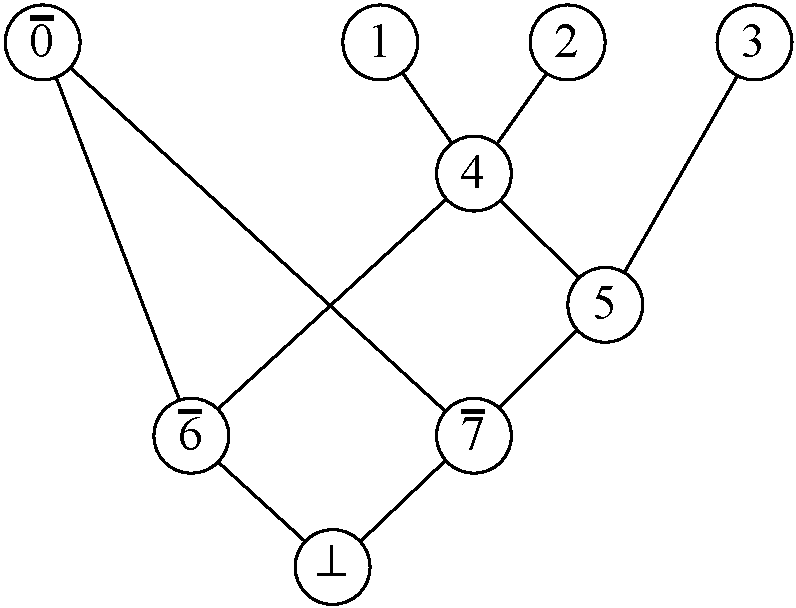
\includegraphics[scale=0.45]{diagrams/paar-ref-graph.pdf}}\]
%
ATP proofs usually identify formulas (typically clauses) by numbers: for
example, the conjecture might be called 0, the axioms might be numbered 1, 2,
\ldots, 250, and new derivations might be called 251 and above. In this paper,
we abstract the ATP proofs by ignoring the actual formulas and just keeping the
numbers. Also, for our own convenience, we put a bar on top of the negated
conjecture and all the formulas derived directly or indirectly from it, denoting
negation. To unnegate the conjecture, or negate any of the steps that are
\emph{tainted} by the negated conjecture, we simply remove the bar. For the last
step, we write $\bot$ rather than $\B{\top}$.

\paragraph{Proof trees.} Proof trees are the standard notation for natural
deduction proofs. For example, the proof graph above is captured by the
following proof tree:
%
\begin{prooftree}
\AXC{$[\B{0}]$}
\UIC{$\B{0}$}
    \AXC{$1$}
        \AXC{$2$}
    \BIC{$1 \land 2$}
        \AXC{$1 \land 2 \longrightarrow 4$}
    \BIC{$4$}
\BIC{$\B{0} \land 4$}
    \AXC{$\kern-4em\B{0} \land 4 \longrightarrow \B{6}$}
\BIC{$\B{6}$}
    \AXC{$[\B{0}]$}
    \UIC{$\B{0}$}
        \AXC{$3$}
            \AXC{$1$}
                \AXC{$2$}
            \BIC{$1 \land 2$}
                \AXC{$1 \land 2 \longrightarrow 4$}
            \BIC{$4$}
        \BIC{$3 \land 4$}
            \AXC{$\kern-3em 3 \land 4 \longrightarrow 5$}
        \BIC{$5$}
    \BIC{$\B{0} \land 5$}
        \AXC{$\kern-5em\B{0} \land 5 \longrightarrow \B{7}$}
    \BIC{$\B{7}$}
\BIC{$\B{6} \land \B{7}$}
    \AXC{$\kern-5em\B{6} \land \B{7} \longrightarrow \bot$}
\BIC{$\bot$}
\end{prooftree}
The proof graph notation is more compact, not least because it enables
sharing of subproofs. For that reason, we will prefer them to proof trees.

\paragraph{Isar proofs.} Isar proofs are a linearization of natural deduction
proofs, but unlike proof trees they enable sharing:
%
\begin{quote}
\keyw{proof}\,~\textit{neg\_clausify} \\
\hbox{}\quad \keyw{assume}\, $\B{0}$ \\
\hbox{}\quad \keyw{have}\, $4$ \keyw{\,by\,} (\textit{metis\, }$1$ $2$) \\
\hbox{}\quad \keyw{have}\, $5$ \keyw{\,by\,} (\textit{metis\, }$3$ $4$) \\
\hbox{}\quad \keyw{have}\, $\B{6}$ \keyw{\,by\,} (\textit{metis\, }$\B{0}$ $4$) \\
\hbox{}\quad \keyw{have}\, $\B{7}$ \keyw{\,by\,} (\textit{metis\, }$\B{0}$ $5$) \\
\hbox{}\quad \keyw{show} \kern.03em$\bot$ \keyw{\kern.05em by\,} (\textit{metis\, }$\B{6}$ $\B{7}$) \\ %% TYPESETTING
\keyw{qed}
\end{quote}
%
The above proof is by contradiction. A direct proof of the above in Isar would
be
%
\begin{quote}
\keyw{proof} -- \\
\hbox{}\quad \keyw{have}\, $4$ \keyw{\,by\,} (\textit{metis\, }$1$ $2$) \\
\hbox{}\quad \keyw{have}\, $5$ \keyw{\,by\,} (\textit{metis\, }$3$ $4$) \\
\hbox{}\quad \keyw{have}\, $6 \lor 7$ \keyw{\,by\,} \textit{metis} \\
\hbox{}\quad $\{$\quad \keyw{assume}\, $6$ \\
\hbox{}\qquad\phantom{$\{$}\keyw{have}\, $0$ \keyw{\,by\,} (\textit{metis\, }$4$ $6$)\quad$\}$ \\
\hbox{}\quad \keyw{moreover} \\
\hbox{}\quad $\{$\quad \keyw{assume}\, $7$ \\
\hbox{}\qquad\phantom{$\{$}\keyw{have}\, $0$ \keyw{\,by\,} (\textit{metis\, }$5$ $7$)\quad$\}$ \\
\hbox{}\quad \keyw{ultimately show}\, $0$ \keyw{\,by\,} (\textit{metis\, }`$6 \lor 7$') \\
\keyw{qed}
\end{quote}
We refer to the Isar tutorial \cite{nipkow-2011-isar} for more information on
the Isar syntax.

\paragraph{Shorthand proofs.}
The last proof format we need to review is a shorthand notation for a subset of
Isar proofs. In their simplest form, these shorthand proofs are simply a list of
derivations, where `$a_1, \ldots, a_n \have c$' means ``from $a_1$ and $\ldots$
and $a_n$, we conclude $c$.'' If among the derivation's assumptions $a_j$
we have the previous derivation's conclusion, we can omit the assumption
and write `$a_1, \ldots, a_{j-1}, a_{j+1}, \ldots, a_n \hence c$' (corresponding
to Isar's \keyw{hence} and \keyw{thus} keywords). Depending on whether we use
the abbreviated format, our running example becomes
%
\begin{align*}
1, 2 & \have 4 &
    1, 2 & \have 4 \\
3, 4 & \have 5 &
    3 & \hence 5 \\
\B{0}, 4 & \have \B{6} &
    \B{0}, 4 & \have \B{6} \\
\B{0}, 5 & \have \B{7} &
    \B{0}, 5 & \have \B{7} \\
\B{6}, \B{7} & \have \bot &
    \B{6} & \hence \bot
\end{align*}
%
Each step is essentially a sequent $\Gamma \vdash \varphi$. The assumptions are
either the negated conjecture ($\B{0}$), facts that were proved elsewhere ($1$,
$2$, and $3$), or formulas that were proved in preceding sequents ($4$, $5$,
$\B{6}$, and $\B{7}$). The succedent of the last sequent is empty ($\bot$).

Direct proofs can be done the same way, but they have the constraints that we
may not assume the negated conjecture $\B{0}$ in any of the sequent and that the
last sequent has the conjecture $0$ as succedent. However, in some of the direct
proofs, we will find it useful to introduce case splits, as we had in the Isar
proof above. For example:
%
\[\hbox{\begin{tabular}{@{}p{.5\textwidth}@{}p{.5\textwidth}@{}}
\frm 1, 2 \hav 4 \end
\frx 3 \hen 5 \end
\frm \hav 6, 7 \end
\cases{\begin{tabular}{l|l}
    $\begin{aligned}[t]
      [&6] \\
      4 \hence {} & 0
    \end{aligned}$\enskip\hbox{}&\enskip
    $\begin{aligned}[t] 
      [&7] \\
      5 \hence {} & 0
    \end{aligned}$
  \end{tabular}}
\end{tabular}}\]
The notation in brace is a case split. In general, a case split has the form
\[\left[\begin{tabular}{l|c|l}
  $\begin{aligned}[t]
    [&\Gamma_1] \\
     \Delta_{11} \have {} & \varphi_{11} \\
     & ~\vdots \\
     \Delta_{1k_1} \have {} & \varphi_{1k_1}
    \end{aligned}$\enskip\hbox{}&\enskip
  $\begin{aligned}[t]
    ~\ldots~ \\
    ~\ldots~ \\
	\\
    ~\ldots~
    \end{aligned}$\enskip\hbox{}&\enskip
  $\begin{aligned}[t]
    [&\Gamma_n] \\
     \Delta_{n1} \have {} & \varphi_{n1} \\
     & ~\vdots \\
     \Delta_{nk_n} \have {} & \varphi_{nk_n}
    \end{aligned}$
\end{tabular}
\right]\]
with the requirement that a sequent with the succedent $\Gamma_1,
\ldots, \Gamma_n$ has been proved already. Also, each of the branches
must be a valid proof. The assumptions $[\Gamma_{\!j}]$ may be used to
discharge assumptions in the same branch, just as if they had been
sequents ${} \have \Gamma_{\!j}$. Seen from outside, the case split
expression stands for a sequent with the succedent
$\varphi_{1k_1}, \ldots, \varphi_{nk_n}$.

\section{Introductory Examples}
\label{sec:introductory-examples}

\subsection{A Linear Proof}
\label{sec:a-linear-proof}

We start with a simple proof by contradiction expressed as a proof tree and
using our shorthand notation:
%
\[\hbox{\begin{tabular}{l@{\qquad}l}
\raisebox{-\height}{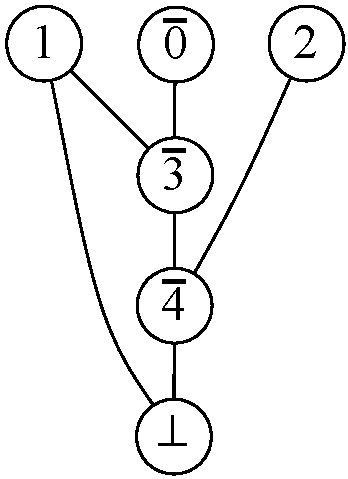
\includegraphics[scale=0.45]{diagrams/linear-ref-graph.pdf}}
&
\qquad
\raisebox{-\height}{$\begin{aligned}[t]
\\
\B 0, 1 & \have \B 3 \\
2, \B 3 & \have \B 4 \\
1, \B 4 & \havebot
\end{aligned}$}
\end{tabular}}\]
Recall from Sect.\ \ref{sec:proof-notations} that the negated conjecture all all
the proof steps that are tainted by it are shown as negated. Next, we turn the
sequents around using contraposition at the sequent level to avoid all
negations. This gives
\begin{align*}
1, 3 & \have 0 \\
2, 4 & \have 3 \\
1 & \have 4
\end{align*}
Finally, if we reorder the sequents and introduce $\hencesym$ wherever possible,
we obtain a direct proof:

\begin{center}
\begin{tabular}{@{}p{.3\textwidth}@{}p{.3\textwidth}@{}}
\begin{tabular}{@{}l@{}}
\keyw{proof} -- \\
\hbox{}\quad \keyw{have}\, $4$ \keyw{\,by\,} \textit{metis} \\
\hbox{}\quad \keyw{hence}\, $3$ \keyw{\,by\,} (\textit{metis\, }$2$) \\
\hbox{}\quad \keyw{thus}\, $0$ \keyw{\,by\,} (\textit{metis\, }$1$) \\
\keyw{qed}
\end{tabular}
&
\begin{tabular}{@{}p{.25\textwidth}@{}p{.25\textwidth}@{}}
\frm \hav 4 \end
\frx 2 \hen 3 \end
\frx 1 \hen 0 \end
\end{tabular}
\end{tabular}
\end{center}

\subsection{Two Lasso-Shaped Proofs}
\label{sec:two-lasso-shaped-proofs}

The next two examples are lasso-shaped proofs:
%
\[\hbox{\begin{tabular}{llll}
\raisebox{-\height}{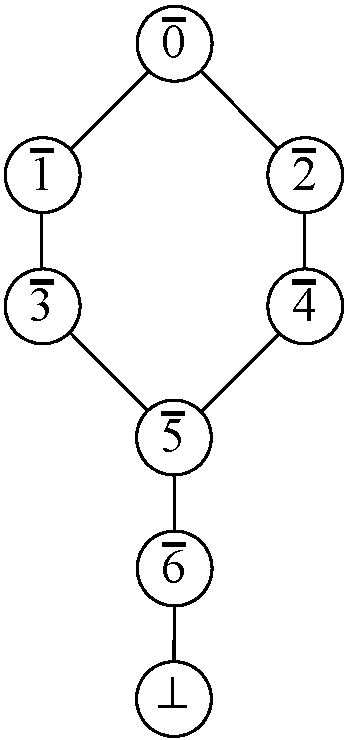
\includegraphics[scale=0.45]{diagrams/lasso-1-ref-graph.pdf}}
&
\qquad
\raisebox{-\height}{$\begin{aligned}[t]
\\
\B 0 & \have \B 1 \\
\B 0 & \have \B 2 \\
\B 1 & \have \B 3 \\
\B 2 & \have \B 4 \\
\B 3, \B 4 & \have \B 5 \\
\B 5 & \have \B 6 \\
\B 6 & \havebot
\end{aligned}$}
&
\qquad\qquad
\raisebox{-\height}{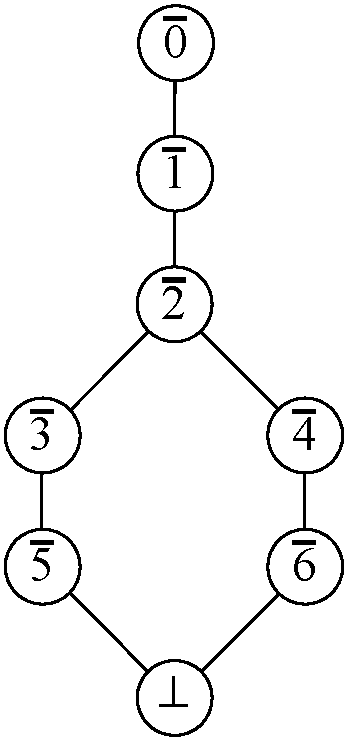
\includegraphics[scale=0.45]{diagrams/lasso-2-ref-graph.pdf}}
&
\qquad
\raisebox{-\height}{$\begin{aligned}[t]
\\
\B 0 & \have \B 1 \\
\B 1 & \have \B 2 \\
\B 2 & \have \B 3 \\
\B 2 & \have \B 4 \\
\B 3 & \have \B 5 \\
\B 4 & \have \B 6 \\
\B 5, \B 6 & \havebot
\end{aligned}$}
\end{tabular}}\]
%
We start with the contradiction proof on the left-hand side. Starting from
$\bot$, it is easy to turn the proof around up to the lasso cycle:
%
\begin{align*}
& \have 6 \\
6 & \have 5 \\
5 & \have 3 \lor 4
\end{align*}
%
When applying the contrapositive to eliminate the negations in $\B 3, \B 4 \have
\B 5$, we obtain a disjunction on the right-hand side of the sequent: $5 \have 3
\lor 4$. To continue from there, we need a case split. Then we can finish then
branches:
%
\[\left[\begin{tabular}{l|l} %% TYPESETTING
    $\begin{aligned}[t]
      [&3] \\
      3 \have {} & 1 \\
      1 \have {} & 0
    \end{aligned}$\enskip\hbox{}&\enskip
    $\begin{aligned}[t] 
      [&4] \\
      4 \have {} & 2 \\
      2 \have {} & 0
    \end{aligned}$
  \end{tabular}\right]\]

The second lasso example is more tricky, because the cycle occurs near the end
of the contradiction proof. Already when redirecting the last inference, we get
a disjunction:
%
\begin{align*}
& \have 5 \lor 6
\end{align*}
%
And if we split naively and finish each branch independently of each other,
we end up with a fair share of duplication:
\pagebreak[3]
\[\left[\begin{tabular}{l|l} %% TYPESETTING
    $\begin{aligned}[t]
      [&5] \\
      5 \have {} & 3 \\
      3 \have {} & 2 \\
      2 \have {} & 1 \\
      1 \have {} & 0 \\
    \end{aligned}$\enskip\hbox{}&\enskip
    $\begin{aligned}[t] 
      [&6] \\
      6 \have {} & 4 \\
      4 \have {} & 2 \\
      2 \have {} & 1 \\
      1 \have {} & 0 \\
    \end{aligned}$
  \end{tabular}\right]\]

In this case, the key is to observe that it is enough if both branches prove
$2$, and from there we prove the rest. The complete proof is (without and
with $\hencesym$):
\[\hbox{\begin{tabular}{@{}p{.25\textwidth}@{}p{.25\textwidth}@{}}
\frm \hav 5 \lor 6 \end
\cases{\begin{tabular}{l|l}
    $\begin{aligned}[t]
      [&5] \\
      5 \have {} & 3 \\
      3 \have {} & 2
    \end{aligned}$\enskip\hbox{}&\enskip
    $\begin{aligned}[t] 
      [&6] \\
      6 \have {} & 4 \\
      4 \have {} & 2
    \end{aligned}$
  \end{tabular}}
\frm 2 \hav 1 \end
\frm 1 \hav 0 \end
\end{tabular}\begin{tabular}{@{}p{.25\textwidth}@{}p{.25\textwidth}@{}}
\frm \hav 5 \lor 6 \end
\cases{\begin{tabular}{l|l}
    $\begin{aligned}[t]
      [&5] \\
      \hence {} & 3 \\
      \hence {} & 2
    \end{aligned}$\enskip\hbox{}&\enskip
    $\begin{aligned}[t] 
      [&6] \\
      \hence {} & 4 \\
      \hence {} & 2
    \end{aligned}$
  \end{tabular}}
\frx 2 \hen 1 \end
\frx \hen 0 \end
\end{tabular}}\]

%Refer to $\eta$ rule or whatever.

Here we were lucky because we could join both branches the node 2 to avoid all
duplication. If we want to stick to a strick no-duplication policy, in general
we sometimes need to join on a disjunction $\varphi_1 \lor \cdots \lor
\varphi_n$, as the next example will illustrate.

\subsection{A Diabolical Proof}
\label{sec:a-diabolical-proof}

Our final example is truly diabolical (and sightly unrealistic):
%
\[\hbox{\begin{tabular}{llll}
\raisebox{-\height}{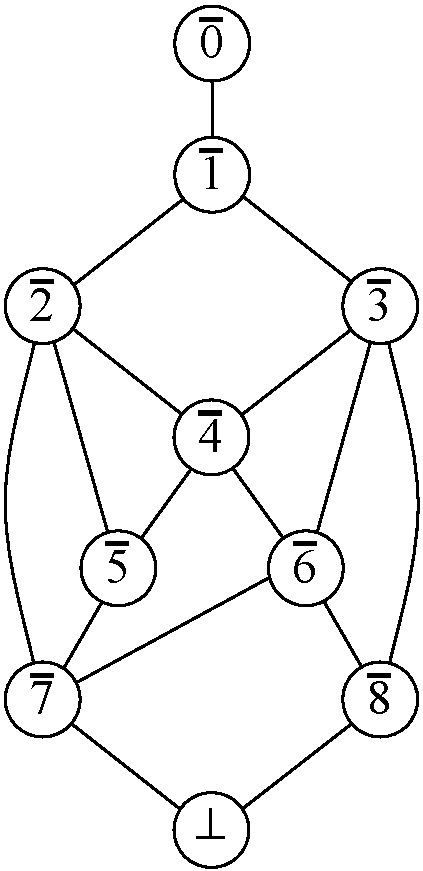
\includegraphics[scale=0.45]{diagrams/diabolical-ref-graph.pdf}}
&
\qquad
\raisebox{-\height}{$\begin{aligned}[t]
\\
\B 0 & \have \B 1 \\
\B 1 & \have \B 2 \\
\B 1 & \have \B 3 \\
\B 2, \B 3 & \have \B 4 \\
\B 2, \B 4 & \have \B 5 \\
\B 3, \B 4 & \have \B 6 \\
\B 2, \B 5, \B 6 & \have \B 7 \\
\B 3, \B 6 & \have \B 8 \\
\B 7, \B 8 & \havebot
\end{aligned}$}
\end{tabular}}\]
%
We start with the contrapositive of the last sequent:
%
\[\have 7 \lor 8\]
%
Then we identify the nodes that dominate only one branch in the refutation graph
(i.e., that are reachable by navigating upward). Looking at the graph, we see
that $\B 5$ dominates $\B 7$ but not $\B 8$, and is the only such node. We
perform a case split and allow ourselves to perform inferences requiring 5 and 7
in the left branch and 8 in the right branch. First the right branch:
%
\begin{align*}
[&8] \\
8 \have {} & 3 \lor 6
\end{align*}
%
There is nothing more we can do for now: Any further inferences we would do in
the right branch would need to be repeated in the left branch. Now we do the
left branch:
%
\begin{align*}
[&7] \\
7 \have {} & 2 \lor 5 \lor 6
\end{align*}
We would now like to perform the inference $5 \have 2 \lor 4$. This requires
a case split:
%
\[\hbox{\begin{tabular}{@{}p{.5\textwidth}@{}p{.5\textwidth}@{}}
\cases{\begin{tabular}{l|r@{}l|l}
 & [&5] & \\
{[2]} & $5 \have {}$ & $2 \lor 4$ & [6]
\end{tabular}}\end{tabular}}\]
%
The 2 and 6 subbranches are left alone. Since only one branch of the subcase
split is nontrivial, we find it more aesthetically pleasing to abbreviate it to
%
\[2 \lor 5 \lor 6 \have 2 \lor 4 \lor 6\]
%
Hence, the left branch proves $2 \lor 4 \lor 6$, the right branch proves $3 \lor
6$, and both branches together prove $2 \lor 3 \lor 4 \lor 6$.

This gives us a new case split, but notice that 6 is dominated by 2, 3, and 4.
We start with it:
%
\[\hbox{\begin{tabular}{@{}p{.5\textwidth}@{}p{.5\textwidth}@{}}
\cases{\begin{tabular}{l|l|l|r@{}l}
 &  & & [&6] \\
{[2]} & [3] & [4] & $6 \have {}$ & $3 \lor 4$
\end{tabular}}\end{tabular}}\]
This proves $2 \lor 3 \lor 4$. Since all but one branches are trivial, we
abbreviate it:
\[2 \lor 3 \lor 4 \lor 6 \have 2 \lor 3 \lor 4\]
It might help to think of such steps as ``rewriting'' steps, where
6 is rewritten into $3 \lor 4$. Now, 4 is dominated by 2 and 3, so we perform
another case split:
\[\hbox{\begin{tabular}{@{}p{.5\textwidth}@{}p{.5\textwidth}@{}}
\cases{\begin{tabular}{l|l|r@{}l}
 & & [&4] \\
{[2]} & [3] & $4 \have {}$ & $2 \lor 3$
\end{tabular}}\end{tabular}}\]
And we abbreviate it:
\[2 \lor 3 \lor 4 \have 2 \lor 3\]
We are left with the conclusion $2 \lor 3$. The rest is reminiscent of our
second lasso-shaped proof:
\[\hbox{\begin{tabular}{@{}p{.25\textwidth}@{}p{.25\textwidth}@{}}
\cases{\begin{tabular}{l|l}
    $\begin{aligned}[t]
      [&2] \\
      2 \have {} & 1
    \end{aligned}$\enskip\hbox{}&\enskip
    $\begin{aligned}[t] 
      [&3] \\
      3 \have {} & 1
    \end{aligned}$
  \end{tabular}}
\frm 1 \hav 0 \end
\end{tabular}}\]
%
Putting all of this together (and using $\hencesym$), we get

\begin{quote}
\begin{tabular}{@{}p{.45\textwidth}@{}p{.5\textwidth}@{}}
\begin{tabular}{@{}l@{}}
\keyw{proof} -- \\
\hbox{}\quad \keyw{have}\, $7 \lor 8$ \keyw{\,by\,} \textit{metis} \\
\hbox{}\quad \keyw{moreover} \\
\hbox{}\quad \blkl \keyw{assume}\, $7$ \\
\hbox{}\qquad \keyw{hence}\, $2 \lor 5 \lor 6$ \keyw{\,by\,} \textit{metis} \\
\hbox{}\qquad \keyw{hence}\, $2 \lor 4 \lor 6$ \keyw{\,by\,} \textit{metis}\blkr \\
\hbox{}\quad \keyw{moreover} \\
\hbox{}\quad \blkl \keyw{assume}\, $8$ \\
\hbox{}\qquad \keyw{hence}\, $3 \lor 6$ \keyw{\,by\,} \textit{metis}\blkr \\
\hbox{}\quad \keyw{ultimately have}\, $2 \lor 3 \lor 4 \lor 6$ \keyw{\,by\,} \textit{metis} \\
\hbox{}\quad \keyw{hence}\, $2 \lor 3 \lor 4$ \keyw{\,by\,} \textit{metis} \\
\hbox{}\quad \keyw{hence}\, $2 \lor 3$ \keyw{\,by\,} \textit{metis} \\
\hbox{}\quad \keyw{moreover} \\
\hbox{}\quad \blkl \keyw{assume}\, $2$ \\
\hbox{}\qquad \keyw{hence}\, $1$ \keyw{\,by\,} \textit{metis}\blkr \\
\hbox{}\quad \keyw{moreover} \\
\hbox{}\quad \blkl \keyw{assume}\, $3$ \\
\hbox{}\qquad \keyw{hence}\, $1$ \keyw{\,by\,} \textit{metis}\blkr \\
\hbox{}\quad \keyw{ultimately have}\, $1$ \keyw{\,by\,} \textit{metis} \\
\hbox{}\quad \keyw{thus}\, $0$ \keyw{\,by\,} \textit{metis} \\
\keyw{qed}
\end{tabular}
&
\begin{tabular}{@{}p{.25\textwidth}@{}p{.25\textwidth}@{}}
\frm \hav 7 \lor 8 \end
\cases{\begin{tabular}{l|l}
    $\begin{aligned}[t]
      [&7] \\
      \hence {} & 2 \lor 5 \lor 6 \\
      \hence {} & 2 \lor 4 \lor 6
    \end{aligned}$\enskip\hbox{}&\enskip
    $\begin{aligned}[t]
      & \\
      [&8] \\
      \hence {} & 3 \lor 6
    \end{aligned}$
  \end{tabular}}
\frx \hen 2 \lor 3 \lor 4 \end
\frx \hen 2 \lor 3 \end
\cases{\begin{tabular}{l|l}
    $\begin{aligned}[t]
      [&2] \\
      \hence {} & 1
    \end{aligned}$\enskip\hbox{}&\enskip
    $\begin{aligned}[t]
      [&3] \\
      \hence {} & 1
    \end{aligned}$\end{tabular}}
\frx \hen 0 \end
\end{tabular}
\end{tabular}
\end{quote}

\noindent
Which is not too bad, considering the spaghetti we started with.

\section{The Algorithm}
\label{sec:the-algorithm}

The process we applied to the examples in the previous section can be
generalized into an algorithm. The algorithm relies on the proof by
contradiction expressed as a set of sequents, which are turned around using the
contrapositive so that the formulas are unnegated (as we did in all the
examples). It maintains a set of \emph{proved nodes} (initially the empty set)
and a set of \emph{target nodes} that it may proceed to prove (initially the set
of all unnegated nodes). The constructed proof is expressed using the shorthand
notation.

\begin{enumerate}
\item Derive as many sequents as possible with their conclusion in the target set
based on the proved nodes. Each time a sequent is appended to the proof, its
conclusion is added to the set of proved nodes.

\item If all the nodes in the target set are proved, we are done. Otherwise, the
last sequent must be of the form $\Gamma \have c_1 \lor \cdots \lor c_n$ for $n
\ge 2$. Perform an $n$-way case split:%
\footnote{A generalization would be to perform an $m$-way case split, with $m <
n$, on disjuncts. For example, we could do a 3-way case split with $c_1 \lor
c_2$, $c_3$, and $c_4$ as the assumptions instead of breaking all the
disjunctions and doing a 4-way split. This could potentially lead to cleaner
proofs, if the groupings are chosen carefully. We will not explore this avenue
further in this paper.}
\[
\left[\begin{tabular}{c|c|c}
$[c_1]$ & $\cdots$ & $[c_n]$ \\
 & & 
\end{tabular}
\right]
\]

\item For each of the branches, invoke the procedure recursively, with the
assumption added to the proved set and with all the nodes that dominate the
branch and no other branch as the target set.

\item After the case split, go back to step 1. The case split itself is seen as
a sequent of the form $\Gamma \have c_1 \lor \cdots \lor c_n$ as far as step 2
is concerned.
\end{enumerate}

Once this procedure has terminated, we abbreviate case splits in which all
but one branch are trivial using ``rewriting,'' transforming
\[
\left[\begin{tabular}{c|c|c|r@{}l|c|c|c}
&&& $[$ & $c_i]$ &&& \\
&&& $\Delta_1 \have {}$ & $d_1$ &&& \\
&&&& $\vdots$ &&& \\
$[c_1]$ & $\cdots$ & $[c_{i-1}]$ & $\Delta_n \have {}$ & $d_n$ & $[c_{i+1}]$ & $\cdots$ & $[c_m]$
\end{tabular}
\right]
\]
into
\begin{align*}
\Delta_1 \have {} & c_1 \lor \cdots \lor c_{i-1} \lor d_1 \lor c_{i+1} \lor \cdots c_m \\
& \vdots \\
\Delta_n \have {} & c_1 \lor \cdots \lor c_{i-1} \lor d_n \lor c_{i+1} \lor \cdots c_m \\
\end{align*}
This works even if the $c_i$ branch has case splits. What we are doing
effectively is taking the nontrivial branch and adding $c_1, \ldots, c_{i-1},
c_{i+1}, \ldots, c_m$ as disjuncts in the conclusions.

Finally, we clean up the proof by introducing $\hencesym$ and translate it to
Isar.

%There is one more concept that needs to be explained: that of a
%``target''. The target set is a set of formulas whose disjunction is
%what we want to prove. For the top-level proof, the target is the
%singleton consisting only of the conjecture. For subproofs, the target
%
%Our approach is based on four basic tools: contraposition (on
%sequents), cut, case split, and ``rewriting.'' Before we look at the
%actual algorithm, it will help to see these tools in action.
%
%Cut (our second tool) is implicit in this notation. The proof
%tree makes it explicit:
%%
%\begin{prooftree}
%\AXC{\phantom{.}}
%\UIC{${} \have 2$\strut}
%  \AXC{\phantom{.}}
%  \UIC{$2 \have 1$\strut}
%\RL{\textsc{Cut}}
%\BIC{${} \have 1$\strut}
%  \AXC{\phantom{.}}
%  \UIC{$1 \have 0$\strut}
%\RL{\textsc{Cut}}
%\BIC{${} \have 0$\strut}
%\end{prooftree}
%
%In general, reordering might not suffice. For example, for the proof
%by contradiction used as the running example in
%Section~\ref{sec:proof-notations}, the contrapositive sequents are
%%
%\begin{align*}
%1, 2 & \have 4 \\
%3, 4 & \have 5 \\
%4, 6 & \have 0 \\
%5, 7 & \have 0 \\
%{} & \have 6, 7
%\end{align*}
%
%We can start outputing the proof
%%
%\begin{align*}
%1, 2 & \have 4 \\
%3, 4 & \have 5 \\
%{} & \have 6, 7
%\end{align*}
%%
%but then we get stuck: There is no obvious way to use the remaining
%two sequents, $4, 6 \have 0$ and $5, 7 \have 0$, because we only know
%``$6$ or $7$.'' With a case split (our third tool), we can finish the
%proof. In the left branch, we assume $6$, which allows us to use the
%sequent $4, 6 \have 0$ to deduce $0$, and similarly in the right
%branch. We saw the full proof in Section~\ref{sec:proof-notations}.
%Case split can be seen as a special case of a multi-cut rule.
%
%Alternative: Using ``rewriting'' (our fourth tool), the sequent ${}
%\have 6, 7$ can be transformed until we reach the desired conclusion.
%E.g.
%%
%\begin{align*}
%4 & \have 0, 7 \\
%4, 5 & \have 0
%\end{align*}
%
%This is justified by the following proof tree:
%%
%\begin{prooftree}
%\AXC{${} \have 6, 7$\strut}
%  \AXC{$4, 6 \have 0$\strut}
%\RL{\textsc{Cut}}
%\BIC{$4 \have 0, 7$\strut}
%  \AXC{$5, 7 \have 0$\strut}
%\RL{\textsc{Cut}}
%\BIC{$4, 5 \have 0$\strut}
%\end{prooftree}
%%
%However, in this case, we prefer the case split, because it more
%clearly reflects the structure of the underlying proof. As the proof
%tree indicates, rewriting is again an instance of cut.

%\section{Theoretical Properties}
%\label{sec:theoretical-properties}
%
%\subsection{Soundness}
%
%  contrapositive
%  MCut
%
%\subsection{Termination}
%
%\subsection{Linear Complexity}
%
%\section{Gallery}
%\label{sec:gallery}
%
%* soundness and completeness are nice, but what matters is that the
%  results are somehow aesthetically pleasing
%* saw few examples of certain shapes
%* actual proof from \textit{Metis\_Examples} (or elsewhere?)
%
%\subsection{Big O Notation}
%
%
%\subsection{Typed Set Theory}
%
%
%\subsection{Tarski}
%

\section{Conclusion}
\label{sec:conclusion}

We presented a method to transform proofs by contradiction as returned by
resolution provers into direct proofs. This sometimes introduces case splits,
but our procedure avoids duplicating proof steps in the different branches of
the split by joining again as early as possible. The result is direct Isar
proofs that have some of the structure Isabelle users have come to expect. Our
approach is fairly simple, it would not surprise us if it were part of folklore
or a special case of existing work.

In a second step, we are interested in transformations that increase proof
readability, such as those available for Mizar proofs \cite{pak-2010}. We also
need to address other issues not treated satisfactorily in Sledgehammer
\cite{paulson-susanto-2007}, notably Skolemization.

\paragraph{Acknowledgment.}
I want to thank Tobias Nipkow, Geoff Sutcliffe, and Joseph Urban for motivating
me to look into this. I am also thankful to Andrei Popescu, who with his deep
theoretical insights helped simplify the approach considerably.

\bibliography{bib}{}
\bibliographystyle{abbrv}

\end{document}
